\reportsection{Appendix}

\subsection{The originating RFC}
\label{app:rfc}

This work began as implementation work around open feature requests against the
\textsf{Arkworks/crypto-primitives} Merkle tree: simplify the split hash interface, remove
caller-side ordering footguns, support richer tree shapes, and compress multi-openings.
Read together, those requests pointed to one broader issue.  The implementation had many
locally reasonable decisions, but no single specification against which their combined
behaviour could be reviewed.

\subsection{CoSet pruning}
\label{app:coset}

The book~\cite{CY26} states the optimisation as $\MTSymbol.\mathsf{CoSet}$.  Working layer
by layer, for each opening we look at the nodes for a single proof and apply two
optimisations: deduplication, and exclusion of computable nodes.

\Cref{fig:coset-example} works the case of openings $\{2,5\}$ on a $16$-symbol tree whose
leaves each hold a coset of two symbols, so index $2$ is carried by leaf $I$ and index $5$
by leaf $J$.  The two single-index co-paths are
\[
  \mathsf{CoPath}(I)=[H,E,C],\qquad \mathsf{CoPath}(J)=[K,D,C].
\]
Deduplication removes the second copy of $C$, which both paths need.  Exclusion removes
$D$ and $E$, because each is computable by the verifier: $D$ is the hash of $H$ and the
opened leaf $I$, and $E$ is the hash of the opened leaf $J$ and $K$.  The proof is
therefore $[H,K,C]$, three nodes against the six that two separate authentication paths
would carry.

Knowing which vertices matter leaves the question of how to label them, and we
implemented and benchmarked both answers.  \code{CoSet} carries explicit vertex labels.
\code{ImplicitCoPath} derives the same labels from the opened indices, performing the same
pruning without materialising a coordinate bookkeeping layer.  The
\code{Committed}/\code{OpeningProof}/\code{Opening} split that came with them makes
ordering and duplicate-index validation part of construction.
\Cref{fig:coset-compression} gives the measurement, and the benchmark harnesses built to
take it prefigure the cost benchmarks of \cref{sec:cost}.

\begin{figure}[t]
  \centering
  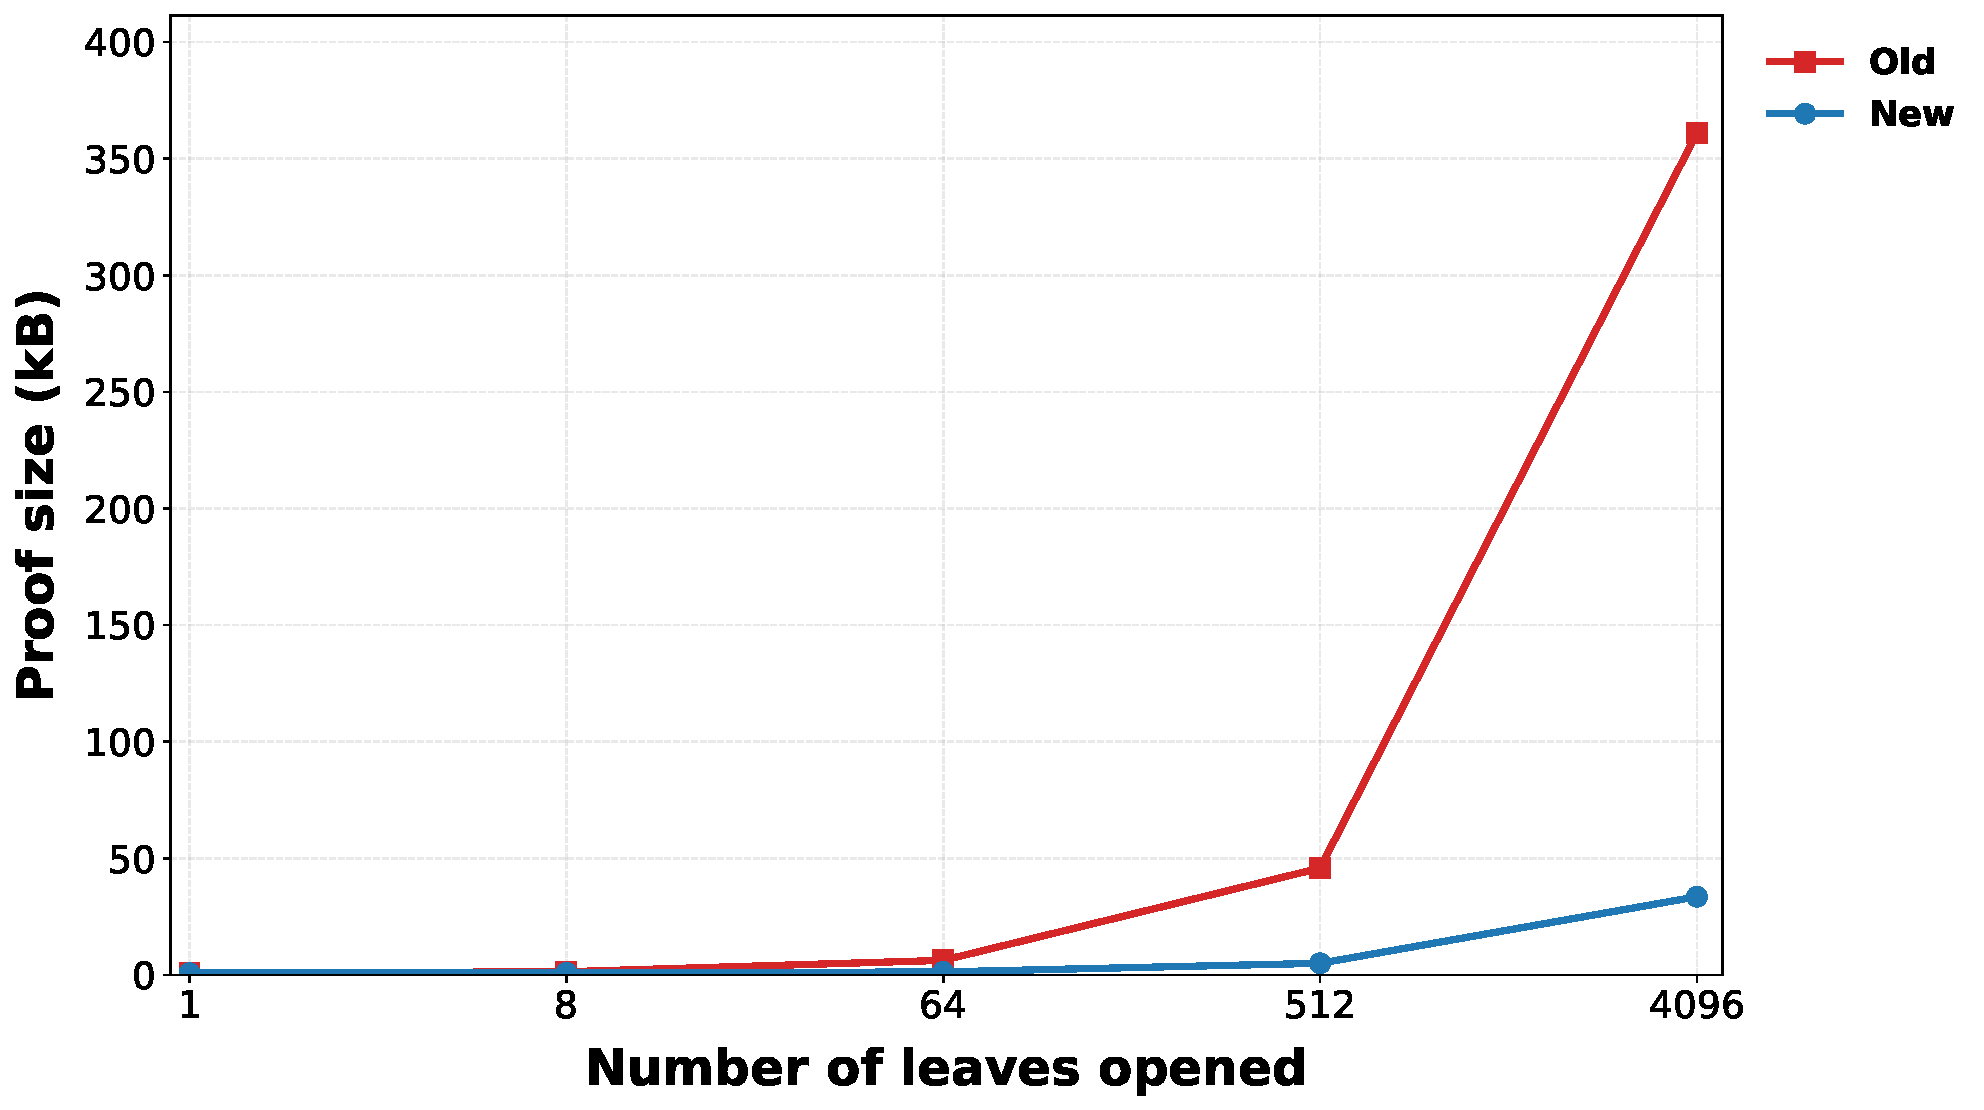
\includegraphics[width=0.5\linewidth]{figures/coset-proof-size-clustered.pdf}
  \caption{Phase-1 multiproof compression on clustered openings of a
  $4{,}096$-leaf tree.  The \code{CoSet} encoding prunes shared path material,
  so proof size tracks the size of the disclosed frontier.  At $4{,}096$ opened leaves
  the compressed proof is
  roughly $33$\,kB against roughly $360$\,kB uncompressed.}
  \label{fig:coset-compression}
\end{figure}

\begin{figure}[t]
  \centering
  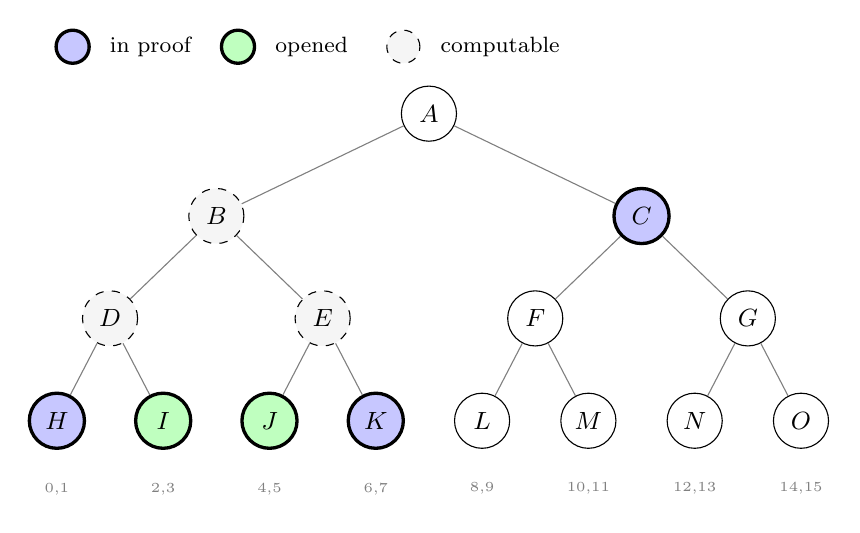
\begin{tikzpicture}[
    lvl/.style={draw,circle,minimum size=7mm,inner sep=0pt,font=\small},
    sent/.style={lvl,fill=blue!22,very thick},
    open/.style={lvl,fill=green!25,very thick},
    comp/.style={lvl,dashed,fill=gray!8},
    plain/.style={lvl,fill=white},
    ed/.style={draw,-,gray}
  ]
  %% leaves, each holding a coset of two symbols
  \node[sent]  (H) at (0.00,0) {$H$};
  \node[open]  (I) at (1.35,0) {$I$};
  \node[open]  (J) at (2.70,0) {$J$};
  \node[sent]  (K) at (4.05,0) {$K$};
  \node[plain] (L) at (5.40,0) {$L$};
  \node[plain] (M) at (6.75,0) {$M$};
  \node[plain] (N) at (8.10,0) {$N$};
  \node[plain] (O) at (9.45,0) {$O$};
  \foreach \n/\a/\b in {H/0/1,I/2/3,J/4/5,K/6/7,L/8/9,M/10/11,N/12/13,O/14/15}
    \node[font=\tiny,gray] at ([yshift=-5mm]\n.south) {\a,\b};
  %% level 2
  \node[comp]  (D) at (0.675,1.3) {$D$};
  \node[comp]  (E) at (3.375,1.3) {$E$};
  \node[plain] (F) at (6.075,1.3) {$F$};
  \node[plain] (G) at (8.775,1.3) {$G$};
  %% level 1
  \node[comp] (B) at (2.025,2.6) {$B$};
  \node[sent] (C) at (7.425,2.6) {$C$};
  %% root
  \node[plain] (A) at (4.725,3.9) {$A$};
  \foreach \p/\c in {D/H,D/I,E/J,E/K,F/L,F/M,G/N,G/O,B/D,B/E,C/F,C/G,A/B,A/C}
    \draw[ed] (\p) -- (\c);
  %% legend
  \node[sent,scale=0.6]  (lg1) at (0.2,4.75) {};
  \node[font=\footnotesize,anchor=west] at (0.55,4.75) {in proof};
  \node[open,scale=0.6]  (lg2) at (2.3,4.75) {};
  \node[font=\footnotesize,anchor=west] at (2.65,4.75) {opened};
  \node[comp,scale=0.6]  (lg3) at (4.4,4.75) {};
  \node[font=\footnotesize,anchor=west] at (4.75,4.75) {computable};
  \end{tikzpicture}
  \caption{CoSet pruning for openings $\{2,5\}$.  Each leaf holds a coset of two
  symbols, so the openings are carried by leaves $I$ and $J$.  Deduplication keeps one
  copy of $C$, and $D$, $E$, and $B$ are excluded as computable from the opened leaves
  and the nodes already sent.  The proof is $[H,K,C]$.}
  \label{fig:coset-example}
\end{figure}

\subsection{Prefix pruning}
\label{app:prefix}

Prefix encoding is the baseline pruning algorithm in \textsf{Arkworks/crypto-primitives}.  It
constructs the full authentication path for every opened index and then compresses each
path against its immediate predecessor:

\begin{enumerate}[itemsep=0pt,topsep=2pt]
  \item Initialise the set of leaf indices $\idxset$.
  \item For each index $i_t\in\idxset$, add the sibling of $i_t$ to the proof $\opening$
  and let $P_t$ be the full authentication path of $i_t$.
  \item Set $\mathit{prefix\_len}_t\leftarrow|\mathrm{lcp}(P_{t-1},P_t)|$ and
  $\mathit{suffix}_t\leftarrow P_t[\mathit{prefix\_len}_t{:}]$.
  \item Add $\mathit{prefix\_len}_t$ and $\mathit{suffix}_t$ to $\opening$.
\end{enumerate}

Two properties follow.  The encoding pays for full paths even where many of them overlap,
and it assumes a previous path in a fixed order, which leaves the encoding ambiguous
unless that order is pinned by the caller.  CoSet pruning reaches the same set of
necessary nodes without either property, which is what \cref{sec:contributions} reports as
the proof-size win.

\subsection{Binding for a general Merkle shape}
\label{app:binding-generic}

\Cref{thm:binding-cr} is stated in \cref{sec:binding} for a perfect binary tree, which is
the case Chiesa and Yogev prove directly~\cite{CY26}.  The same bound holds over a general
Merkle shape $G_\ell$, and this section gives that argument.

The argument runs through three lemmas.

\begin{lemma}[Birthday bound]\label{lem:birthday}
Let $\ROFunction$ be drawn uniformly from the functions into $\bits^{\digestbits}$, and
suppose $\querybudget$ distinct inputs are queried.  The probability that two of the
answers coincide is at most $\querybudget(\querybudget-1)/2^{\digestbits+1}$.
\end{lemma}

\noindent\emph{Proof.}
The $\querybudget$ answers are independent and uniform on $\bits^{\digestbits}$, because
the inputs are distinct and $\ROFunction$ is uniform.  Fix an unordered pair of query
indices.  Its two answers agree with probability $2^{-\digestbits}$.  There are
$\binom{\querybudget}{2}=\querybudget(\querybudget-1)/2$ such pairs, so a union bound
over them gives
$\querybudget(\querybudget-1)/2\cdot2^{-\digestbits}
=\querybudget(\querybudget-1)/2^{\digestbits+1}$.\hfill$\square$

\begin{lemma}[A break extracts a collision]\label{lem:extract}
Suppose $\MTCheck$ accepts both $(\idxset_0,\MTMessageSubVector_0,\opening_0)$ and
$(\idxset_1,\MTMessageSubVector_1,\opening_1)$ against the same commitment $\comm$, and
the two disagree at some $i\in\idxset_0\cap\idxset_1$.  Then the oracle trace of the
experiment contains two distinct inputs with the same output.
\end{lemma}

\noindent\emph{Proof.}
Acceptance of opening $b$ means the verifier recomputes a labelled path from leaf $i$ to
the root.  Write that path $\ell_0^b,\ell_1^b,\dots,\ell_d^b$, where $\ell_0^b$ is the
leaf label and $\ell_d^b=\comm$.  Each $\ell_0^b$ is the output of a leaf-tagged call on
the encoded symbol at $i$, and each $\ell_{j+1}^b$ is the output of a node-tagged call
whose input contains $\ell_j^b$.

The two openings disagree at $i$, and the leaf encoding is injective, so the two
leaf-tagged calls have distinct inputs.  If $\ell_0^0=\ell_0^1$ those two distinct
inputs already share an output, which is the claimed collision.  Otherwise
$\ell_0^0\neq\ell_0^1$ while $\ell_d^0=\ell_d^1$, so the two label sequences disagree at
level $0$ and agree at level $d$.  Let $j$ be least with $\ell_{j+1}^0=\ell_{j+1}^1$,
which exists because level $d$ agrees.  By minimality $\ell_j^0\neq\ell_j^1$.  Both
paths pass through index $i$, so on both sides $\ell_j^b$ occupies the same child slot of
the level-$(j+1)$ call.  The two level-$(j+1)$ inputs therefore differ while their
outputs agree.  Domain separation makes the colliding pair genuine, because the leaf and
node call families carry distinct tags and this pair is drawn from within one
family.\hfill$\square$

\begin{lemma}[Shape is pinned only by geometry tags]\label{lem:geometry}
If node calls absorb no geometry tag, then two shapes whose roots collide admit openings
that each shape's own verifier accepts against the other's root.  If every leaf and node
call instead absorbs its position as a tag of layer, index, and arity, then a root
accepted under shape $G$ is accepted under a shape $G'\neq G$ only if the trace contains
a collision.
\end{lemma}

\noindent\emph{Proof.}
For the first part, an untagged root is the output of the topmost call and its input
records nothing about the shape that produced it, so any pair of shapes reaching a common
root admits both readings.  The demonstration below exhibits such a pair for arity $2$
against arity $8$.  For the second part, acceptance under $G$ forces, at every position
on the opening path, a call whose input begins with that position's tag under $G$.  A
shape $G'\neq G$ differs from $G$ at some position on the path in layer, index, or arity,
so the corresponding two calls have distinct inputs.  Both outputs are the accepted root,
which is a collision.\hfill$\square$

\noindent\emph{Proof of \Cref{thm:binding-cr}.}
Let $\adv$ win the position-binding experiment, so it outputs $\comm$ with two accepted
openings that disagree at a shared index.  \Cref{lem:extract} converts that pair into two
distinct inputs of the trace sharing an output.  \Cref{lem:geometry} removes the
remaining freedom, since under the stated domain separation any re-reading of the same
digests as a different shape also leaves a collision in the same trace.  Every winning
execution therefore leaves a collision behind, which gives
$\Adv{bind}(\ThetaVC)\le\Pr[\text{oracle-trace collision}]$.  The complete experiment
issues at most $\querybudget$ distinct queries, so \Cref{lem:birthday} bounds that
probability by $\querybudget(\querybudget-1)/2^{\digestbits+1}$.  For the concrete
condition, $\querybudget\le2^{h}$ gives
$\querybudget(\querybudget-1)<2^{2h}$, hence
\[
  \Adv{bind}(\ThetaVC)<\frac{2^{2h}}{2^{\digestbits+1}}=2^{2h-\digestbits-1},
\]
and $2^{2h-\digestbits-1}\le2^{-\secpar}$ holds if and only if
$\digestbits\ge\secpar+1+2h$.\hfill$\square$

The reduction is machine-checked in Lean~4~\cite{ZLeanVC26} for each statement.
\Cref{lem:birthday} is \code{birthdayBound}, proved by union bound over the
$\querybudget(\querybudget-1)/2$ unordered pairs, and specialised to $\digestbits$-bit
digests as \code{birthdayBound\_kappa}.  \Cref{lem:extract} is
\code{mt\_colliding\_paths}, which rests on \code{walkCopath\_inj} for the injectivity needed
to walk upwards in the tree, and its two hypotheses are supplied by
\code{encodeLeaf\_inj} and \code{encodeLeaf\_ne\_encodeNodes}.  The step from a winning
adversary to a trace collision is \code{coupling\_trace\_le\_collisionBound}, and the
closing arithmetic is \code{collisionBound\_le\_inv\_pow}.  The rule is carried as a
decidable definition, \code{MeetsBindingTarget} over
$\digestbits=\code{fieldBits}\cdot\code{digestElems}$, with
\code{meetsBindingTarget\_ofField} discharging it for any field and
\code{babyBear\_meetsBindingTarget} discharging BabyBear with no hypothesis at all.

Two caveats on that scope.  The formalisation closes the singleton-opening case end to
end, and the multi-leaf collision lemma is still in progress, so \Cref{lem:extract} is
mechanised for a single opened index and argued on paper for a general index set.
\Cref{lem:geometry} is not mechanised.  The reduction is otherwise generic over the Merkle
shape, with the binary tree as the exhibited instance, and $k$-ary and arbitrary-length
shapes share the argument without yet being exhibited (\cref{sec:conclusion}).

\subsection{The \code{MerkleHasher} trait}
\label{app:hasher-trait}

Every hasher in \textsf{ark-mt} satisfies one trait, with the digest and salt widths left
as associated types:

\begin{verbatim}
pub trait MerkleHasher: Clone + Send + Sync {
    type Symbol: Clone + Send + Sync;
    type Digest: Clone + Eq + Send + Sync + WireEncode + WireDecode;
    type Salt: Clone + Default + Send + Sync + WireEncode + WireDecode;

    fn sample_salt<R: RngCore + CryptoRng>(&self, rng: &mut R) -> Self::Salt;
    fn hash_leaf(&self, symbol: &Self::Symbol, salt: &Self::Salt) -> Self::Digest;
    fn hash_nodes(&self, children: &[Self::Digest]) -> Self::Digest;
}
\end{verbatim}

The Poseidon2 hasher sets the digest to be the field it is instantiated over, and its
hiding counterpart samples the salt the same way:

\begin{verbatim}
impl<F: PrimeField> MerkleHasher for Poseidon2Hasher<F> {
    type Digest = F;
    ...
}

impl<F: PrimeField + Absorb> MerkleHasher for PoseidonHidingHasher<F> {
    type Salt = F;

    fn sample_salt<R: RngCore + CryptoRng>(&self, rng: &mut R) -> F {
        F::rand(&mut ark_rng_wrapper(rng))
    }
    ...
}
\end{verbatim}

Neither implementation reads the target security parameter $\lambda$.  The digest and salt
widths are whatever the associated types resolve to, fixed once at the type level and never
checked against the field.

\subsection{Why the cost transitions fall where they do}
\label{app:hash-blocks}

\Cref{sec:cost} prices what crossing a permutation or compression-block boundary costs.
This figure is the mechanism behind that step.

\begin{figure}[H]
  \centering
  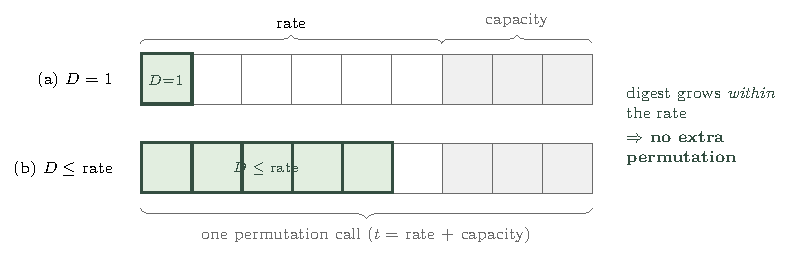
\includegraphics[width=0.42\linewidth]{figures/poseidon-rate-width.pdf}\hfill
  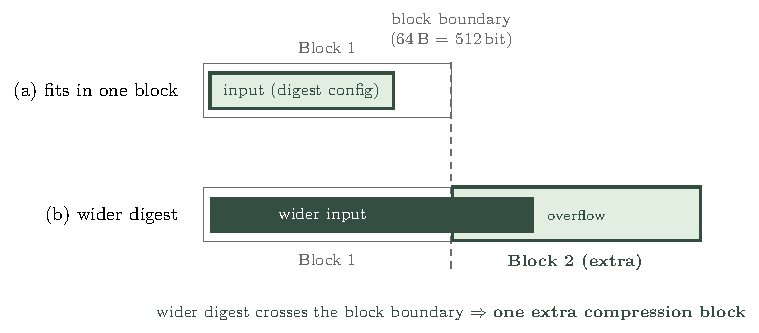
\includegraphics[width=0.42\linewidth]{figures/blake3-extra-block.pdf}
  \caption{Why the cost transitions of \cref{sec:cost} fall where they do.  Left: a
  Poseidon2 permutation writes its output into the rate of a fixed-width state, so widening
  the digest up to the rate stays inside one permutation call and is free.  Right: Blake3
  absorbs in fixed blocks, so a digest that crosses a block boundary costs one extra
  block.}
  \label{fig:hash-blocks}
\end{figure}

\subsection{Bytewise cost curves}
\label{app:bytewise-cost}

The Blake3 counterpart to \cref{fig:poseidon-cost}, in the same triptych format:

\begin{figure}[H]
  \centering
  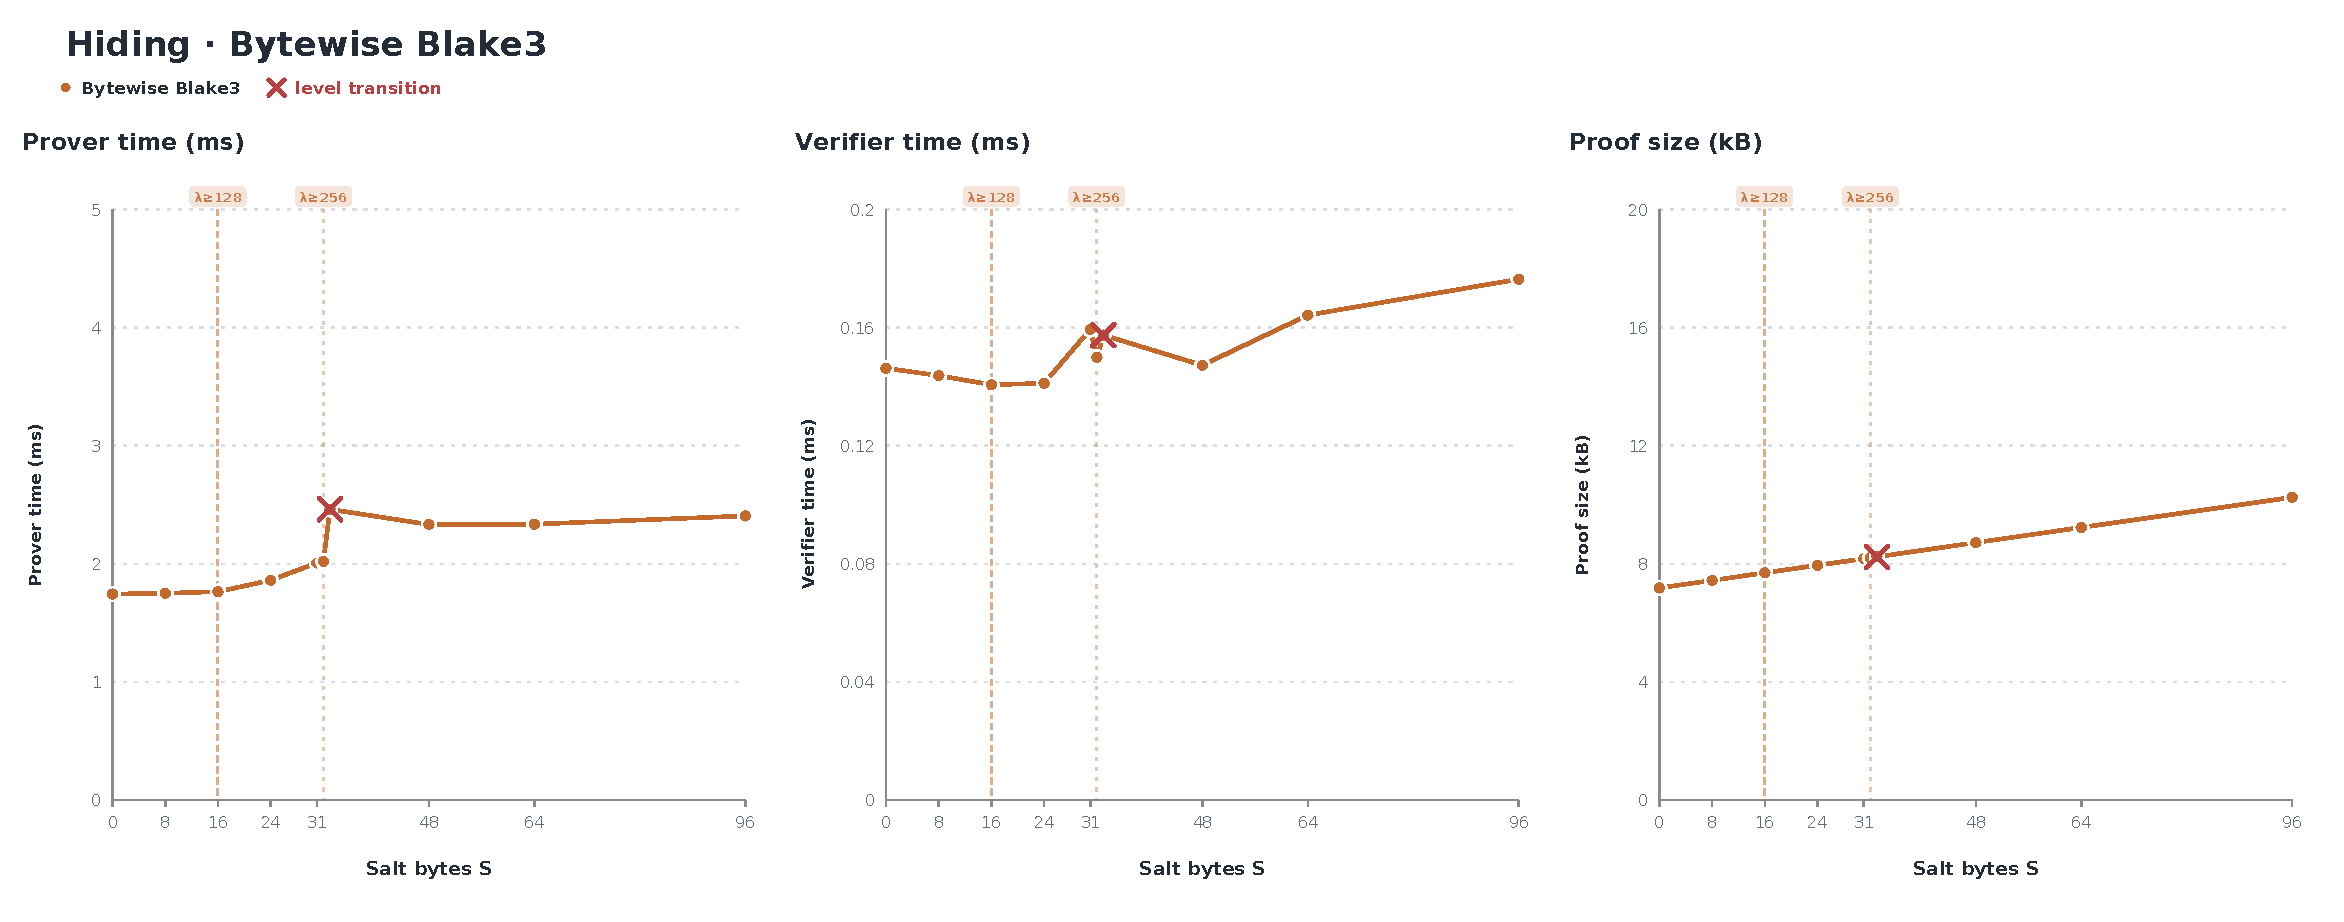
\includegraphics[width=\linewidth]{figures/benchmark_hiding_bytewise_triptych_extra_x.pdf}\\[5pt]
  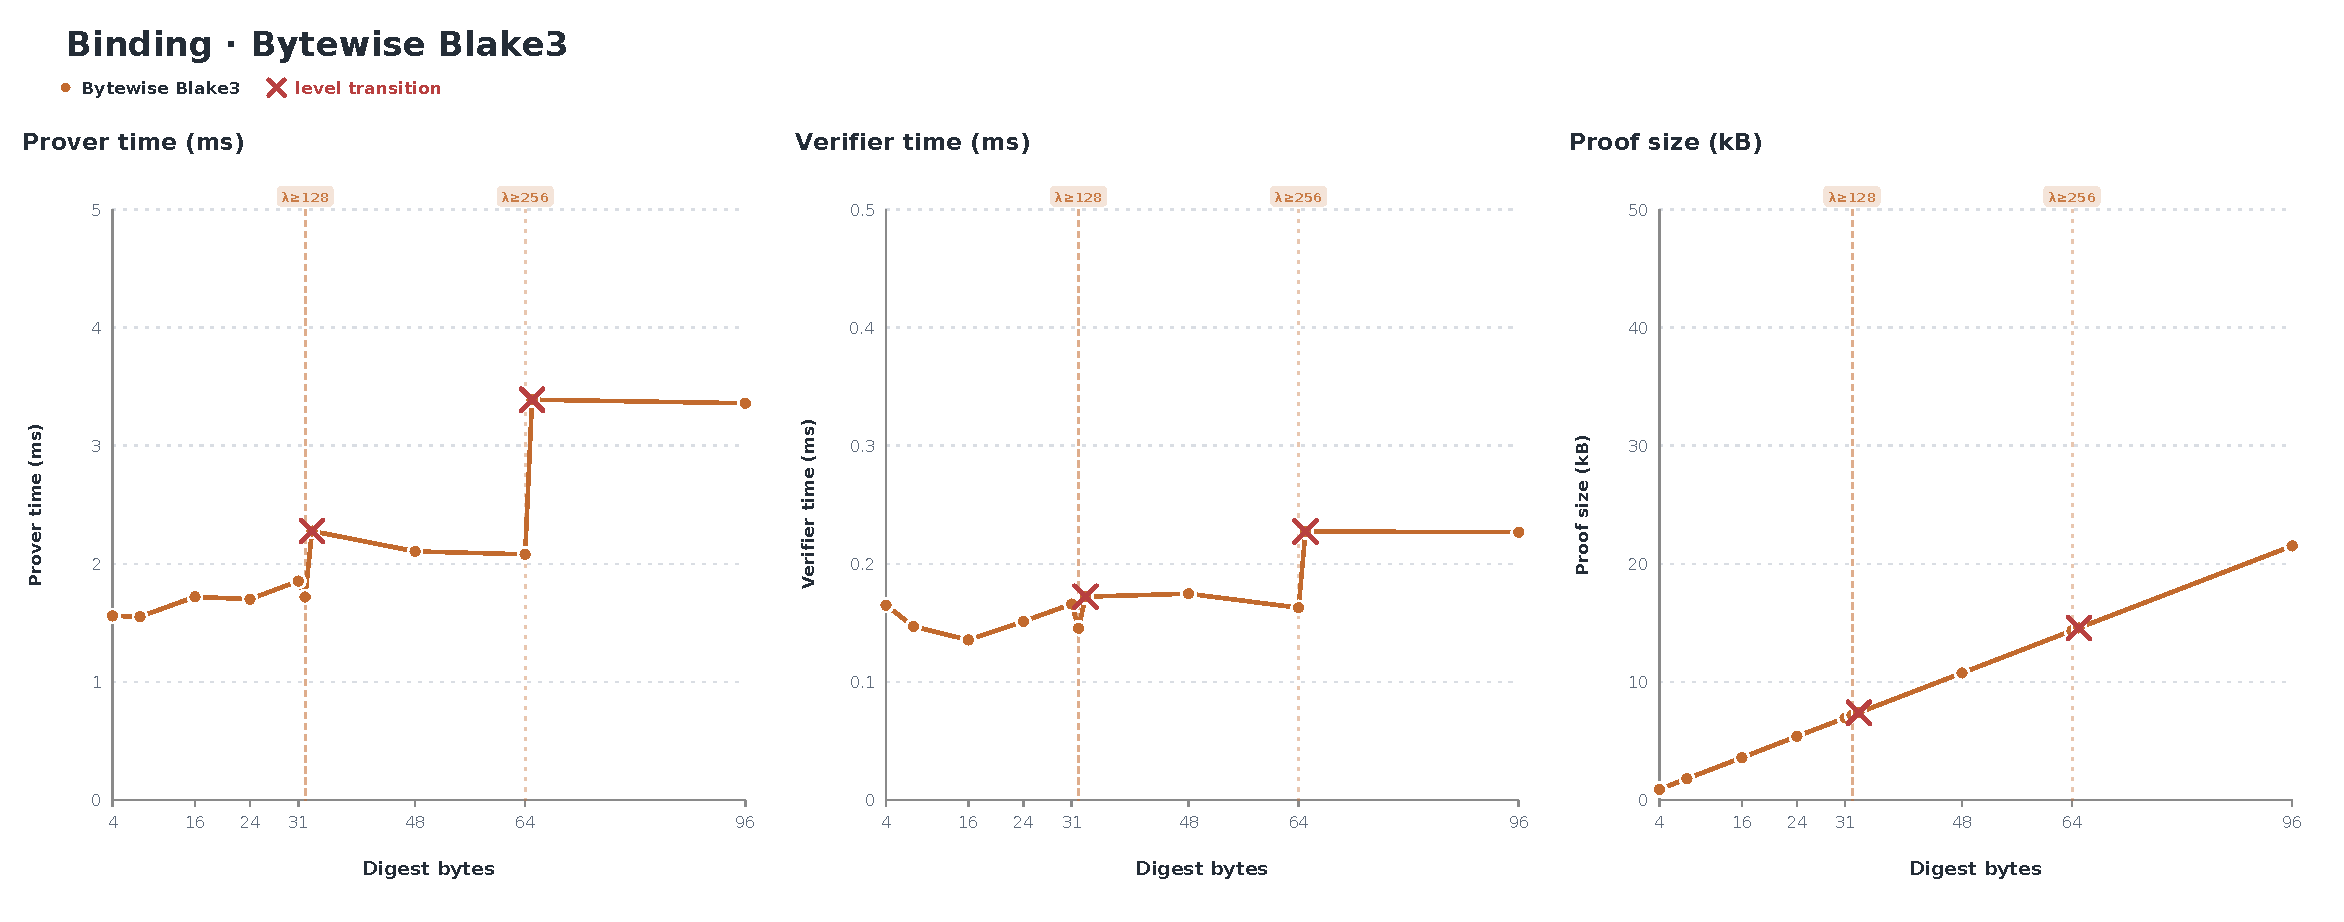
\includegraphics[width=\linewidth]{figures/benchmark_binding_bytewise_triptych_extra_x.pdf}
  \caption{Blake3 hiding cost as salt width grows (top) and binding cost as digest width
  grows (bottom), both measured in bytes.  Markers flag inputs that cross into an extra
  compression block.}
  \label{fig:blake3-cost}
\end{figure}

\subsection{The collision demonstration}
\label{app:demo}

The search of \cref{sec:binding} precomputes the roots of one shape into a table and then
draws from the other until a root repeats:

\begin{verbatim}
let mut binary_roots = HashMap::with_capacity(PRECOMPUTE_BUDGET); // 2^16
for _ in 0..PRECOMPUTE_BUDGET {
    let message = random_message(&mut rng);
    let committed = binary.commit(&message);
    binary_roots.insert(root_key(committed.root()), BinaryCandidate { message });
}
for searched in 1usize.. {
    let kary8_message = random_message(&mut rng);
    let kary8_committed = kary8.commit(&kary8_message);
    if let Some(binary_candidate) = binary_roots.get(&root_key(kary8_committed.root())) {
        // binary_candidate.message and kary8_message now share a root
        ...
    }
}
\end{verbatim}

\subsection{Hiding: the intended reduction}
\label{app:hiding-reduction}

\Cref{prop:salt-card} certifies the salt cardinalities that \cref{sec:hiding} uses.  This
section states the bound they feed into and what remains open.

The cardinalities themselves are machine-checked, as
\code{fieldSalt\_card\_lower\_bound} and \code{byteSalt\_card\_lower\_bound}, with
\code{babyBear\_byte\_salt\_hiding} as the concrete instance~\cite{ZLeanVC26}.  The bound
they feed into remains an \emph{intended reduction}.  The root-hiding obligation has the form
\[
  \Adv{hide}(\ThetaVC)
  \le \frac{\msglen\querybudget}{2^{\saltbits}}
  + \varepsilon_{\mathrm{internal}}(\digestbits,\querybudget,\shape),
\]
where the two terms represent the two bad events, a query to a hidden salted leaf
input, or an internal hash collision as the simulation rebuilds the tree from the
leaves up to the root.  The bound is written against the intended game, in which the
honest experiment samples the oracle jointly with the salts, and discharging that game
is the open step.  The salt-hit term rests on a standard averaging step that is not yet
formalised.  The certified salt cardinalities are prerequisites for this bound and not
the theorem itself, and lifting the result to the selective-opening target is the
composition step after that.

\subsection{Compiled soundness}
\label{app:compilation}

In the compiler that \textsf{ark-vc}~\cite{ArkVC26} targets, each oracle message is committed and the
verifier's queries are answered with authenticated openings.  The root is fixed into
the transcript from the first message, so \emph{binding} enters the compiled soundness
bound additively~\cite{CDGS24}, which is what lets a soundness argument treat each
committed answer as fixed before the query set is chosen.  \emph{Hiding} is what a
zero-knowledge argument relies on across the same compilation, and its error grows only
linearly in the query budget, which is why \cref{sec:hiding} sizes the salt from $\secpar$
alone.  The grinding
adversary that inflates the query budget, and the digest target it forces, are priced
in \cref{sec:binding}.
